% !TEX root = ../../thesis.tex

\cleartoleftpage
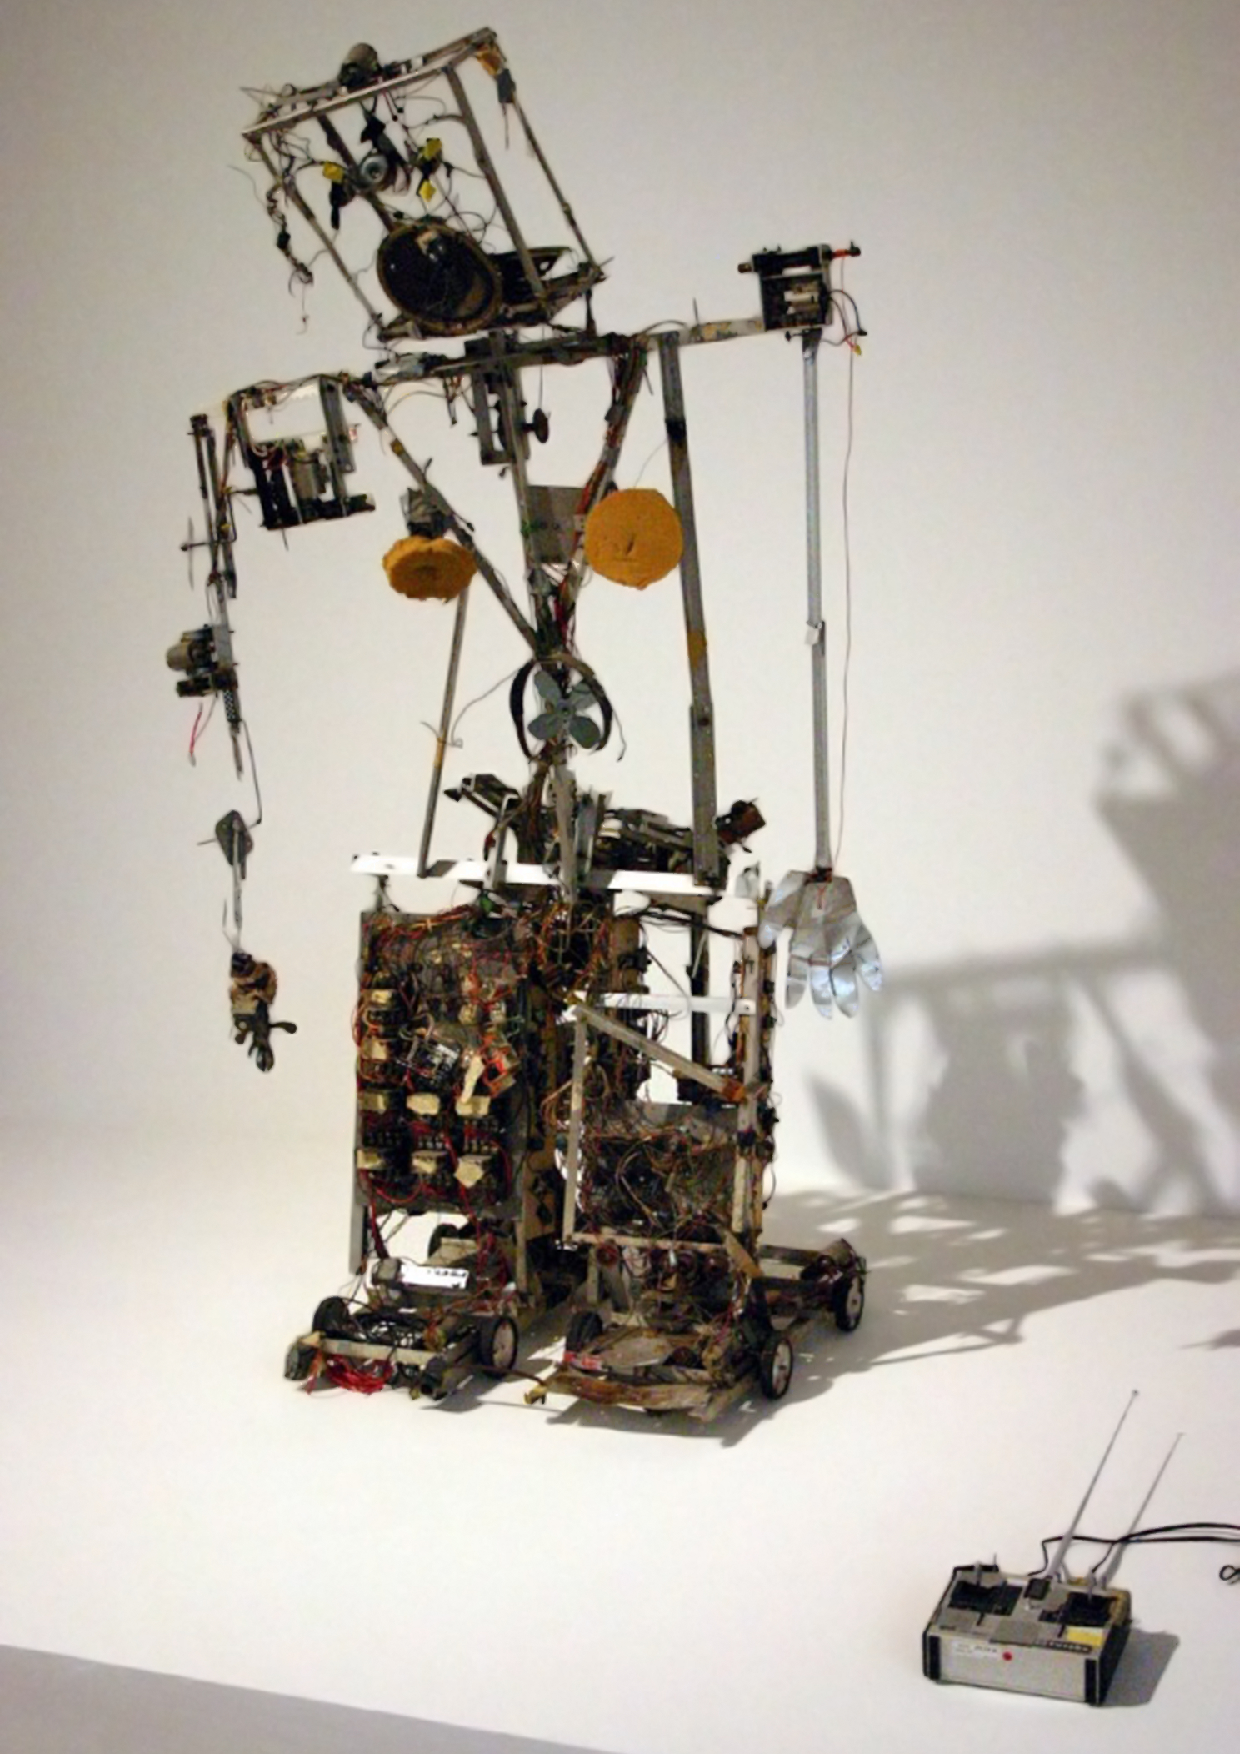
\includepdf{../media/chapter_illustration/Nam_Jun_Paik}

\chapter{Art} % (fold)

\cleanchapterquote{Artists and mathematicians have finally a lot of point in common in the way of working. There is this important role for the mathematician and scientists generally, of inspiration, culture, exchange of ideas, school of thought which change over time or which vary from one country to another, and at the same time, the scientific universality is the same as those found in the arts.}{Cédric Villani}


\section{Introduction} % (fold)

For ages, Science and Art have been mingled. Leonard da Vinci\footnote{Humanist artist who lived during the Renaissance, Leonardo da Vinci had different hat. He was a painter, sculptor and musician but also an engineer, mathematician, physicist, biologist, astrologer, architect and urban planner. Famous today for his painting, he also left visionary flying and war machines.} is a meaningful example of the very existence of such scientific-artist status. Contrary to popular opinion, the two worlds are more agree with each other than opposed. Indeed, in both areas if the methods of investigation and processes implemented to experiment the world may differ, both artists and scientists are motivated toward the same goal: understanding the world around them to share and exchange knowledge with others.


Several results and technologies coming from Science applications have been transformed into material resources, instrumental, or technical processes for Art. As an example, chronophotography invented by Etienne Jules Marey and Eadweard Muybridge to study human and animal locomotion (see \figurename~\ref{fig:marey_chronophotography}) has been a source of inspiration for Futurists\footnote{At the Futurist time, Art seeks to express the dynamism of modern life and the representation of contemporary society: they consider the movement and speed as the most significant emerging phenomena of the twentieth century.} who reproduce in their work the movement decomposition visible in chronophotographies (see \figurename~\ref{fig:duchamp_chronophotography} and \figurename~\ref{fig:russolo_chronophotography}). Futurists are proponents of the fusion of art with technology and the natural sciences: \emph{"The method of constructing a machine is similar to the method of manufacturing a work of art"}~\cite{severini1917machinisme}.


\begin{figure}[!t]
\centering
    \subfloat[][]{\label{fig:marey_chronophotography}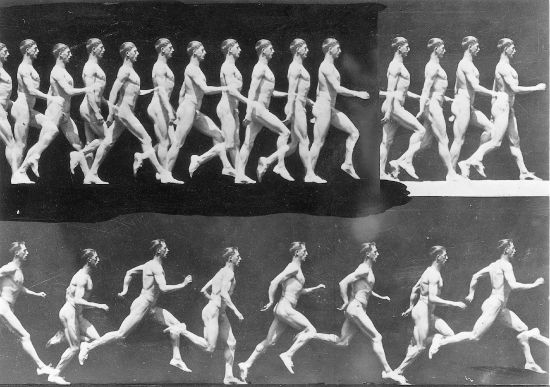
\includegraphics[width=0.8\linewidth]{chronophotography.jpg}}\\
    \subfloat[][Marcel Duchamp, \emph{Nu descendant un escalier}, oil on canvas, 146 x 89 cm (1912) - Philadelphia Museum of Art, Philadelphie (États-Unis).]{\label{fig:duchamp_chronophotography}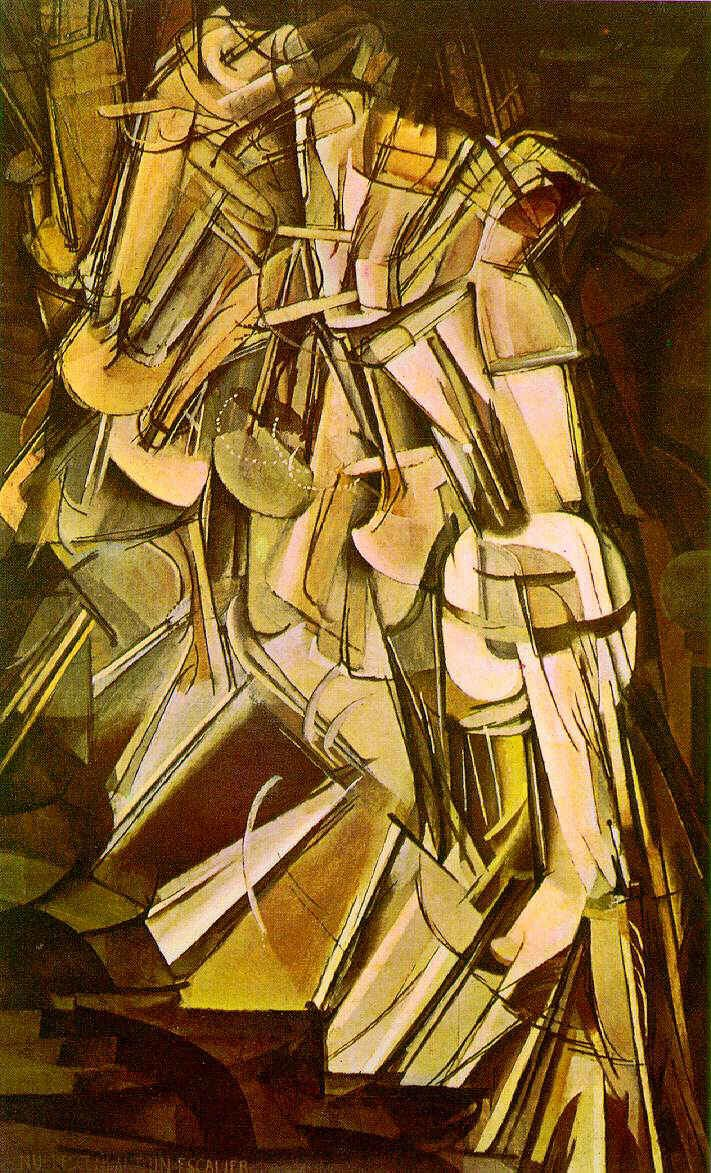
\includegraphics[height=6cm]{chronophotography_duchamp.jpg}}
    \hfil
    \subfloat[][Luigi Russolo, \emph{Dynamisme d’une automobile}, 1912 – Centre Georges Pompidou.]{\label{fig:russolo_chronophotography}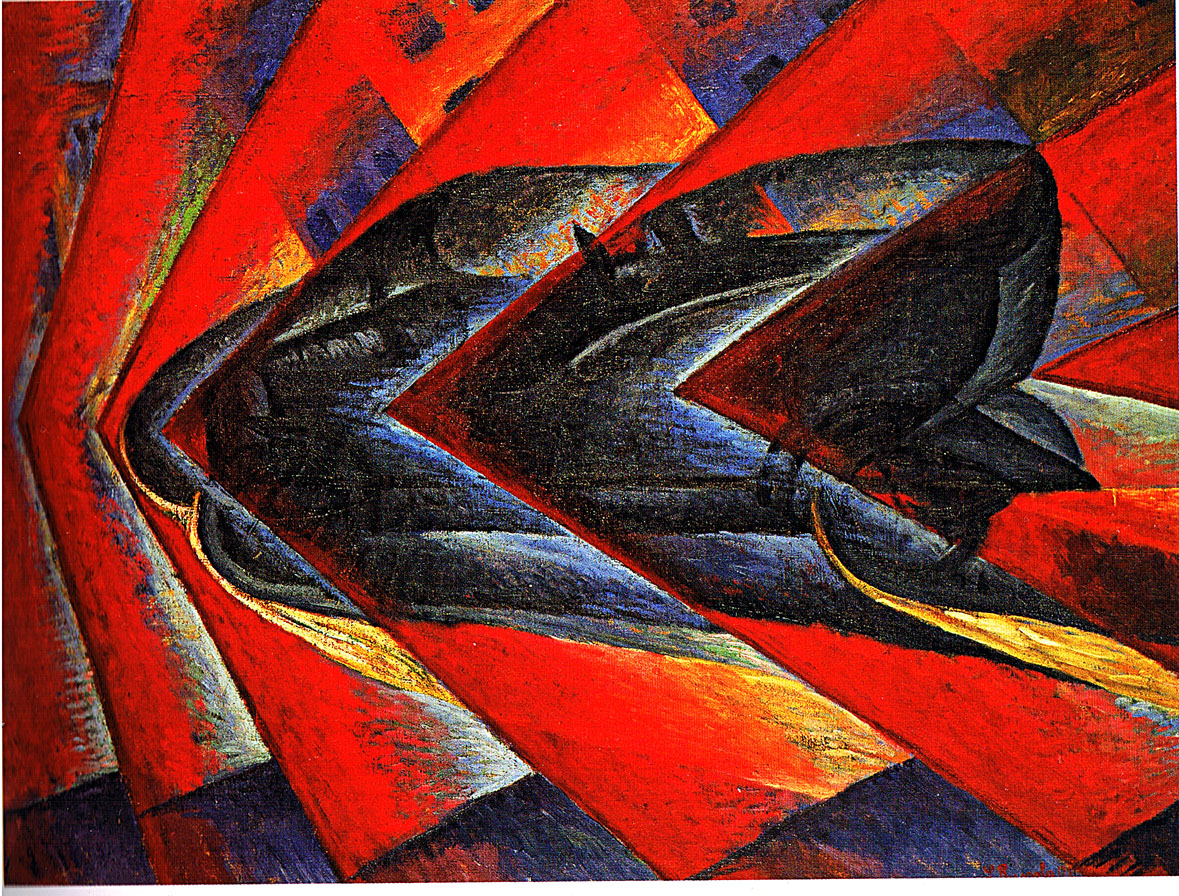
\includegraphics[height=6cm]{chronophotography_russolo.jpg}}
    \caption{}
    \label{fig:chronophotography_history}
\end{figure}


If Science proves to be a source of inspiration for Art, in return, Art is also involved in Science and play a major role in helping the general public to an understandable representation of complex scientific discoveries or concepts. Indeed when mixed with science and technical applications, the artistic creation is also an original vector mediation to reach the uninitiated. The sensory experience brought by a work of art  favors the appropriation of innovative technology or research results, especially because it demystifies the complexity of the mechanisms involved with sensory approach and concrete production more easily comprehensible than theoretical explanations. In doing so it often helps to understand the issues, potential uses, defuse fears of their novelty and expand distribution.
Astrophysics is a great example of such use. None of us will ever see a giant black hole or the sun becoming a red giant. In this context, artists contributions is vital as it would be difficult to get attention and interest needed to the funding of such expansive research without appropriate mediation.


In this direction, the Flowers team in collaboration with the artist and movie-maker David Lynch leads a project called "ergo robots" (see \figurename~\ref{fig:ergo_robot}) whose context is the "Mathematics: A Beautiful Elsewhere"\footnote{Mathematics: A Beautiful Elsewhere is a unique exhibition created by the Fondation Cartier pour l’art contemporain with the aim of offering visitors, to use the mathematician Alexandre Grothendieck’s expression, “a sudden change of scenery.” The Fondation Cartier has opened its doors to the community of mathematicians and invited a number of artists to accompany them. They are the artisans and thinkers, the explorers and builders of this exhibition. More info on \url{http://fondation.cartier.com/en/art-contemporain/26/exhibitions/294/all-the-exhibitions/89/mathematics-a-beautiful-elsewhere/}} exhibition in 2011 at the Cartier Foundation for Contemporary Art. The experience of the Flowers team addressing the artificial curiosity, the embodiment and discovery of language in robots, aimed among other goals, the interaction with a non-science-enthusiast public. In this experiment the collaboration between science and art has revealed the art as a medium and tool for scientific mediation.

\begin{figure}[!t]
\centering
    \subfloat[][]{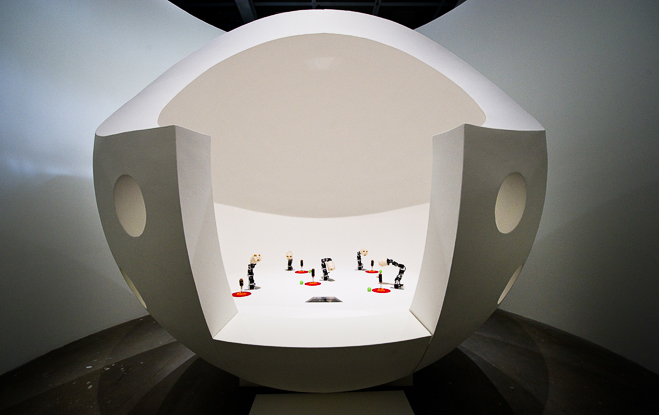
\includegraphics[height=4.2cm]{ErgoRobotFondationCartier.jpg}}
    \hfil
    \subfloat[][]{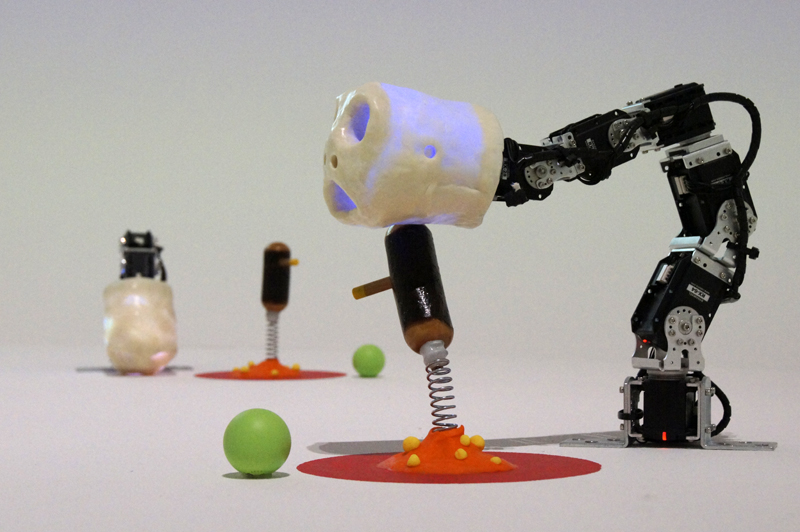
\includegraphics[height=4.2cm]{ErgoRobots13.jpg}}
    \caption{}
    \label{fig:ergo_robot}
\end{figure}


Yet this kind of collaboration between a scientific laboratory and artists are rare.
We can indeed notice the recent increase in complexity and the culture/education level needed to understand the last work coming from these two worlds\footnote{C.P.Snow explained in "two culture" theory (REF) that people in humanities and art, and those in the science had developed a sufficiently different language and world-views that they did not understand each other.}. Without art history knowledge, it is sometimes difficult for a scientist to understand last contemporary work of art. Likewise, it is somehow difficult for artists\footnote{It should be noted that the arts community hosts various artists profiles. Curiously (in many cases), works combining art and science are creations of artists who are none other than scientific converted.} to appreciate the scientific work because of the technical complexity involved.
The interaction is indeed sometimes difficult because we do not speak the same language but robots raise countless issues and challenges and even if some of them are very technical requiring the use of mathematical formalisms to be explored, a wide range of problematic can be addressed with a the relevant collaboration of artists.

What interests us particularly, and responds to this research, is the alternative perspectives artists bring about robot societal impact or human-robot interaction, opening new research axes or new way to explore them.
One of the emblematic case of these loans to art, is the robotic emotion. The expression of emotions in a virtual machine or humanoid holds a double representation: firstly, it depends on how the human emotional functions have been understood; secondly, it is based on a representation of iconography of emotions. These two representations are well mastered by artists. Brilliant examples can be found in the cinema (see \figurename~\ref{fig:robot_emotion_cinema}). Only using basic beep-based sounds, R2D2 is able to communicate and actually is more appealing than C3PO, classic humanoid robot speaking hundreds of languages. Another impressive example is Wall-E, without an actual human face, the animators have been able to create a wide range of intense emotions.
These two examples show how robotists could benefit from artists expertise in the field of sensitive to design more expressive robots.


\begin{figure}[t]
\centering
    \subfloat[][The C3-PO and R2D2 robots in Star Wars: A new hope]{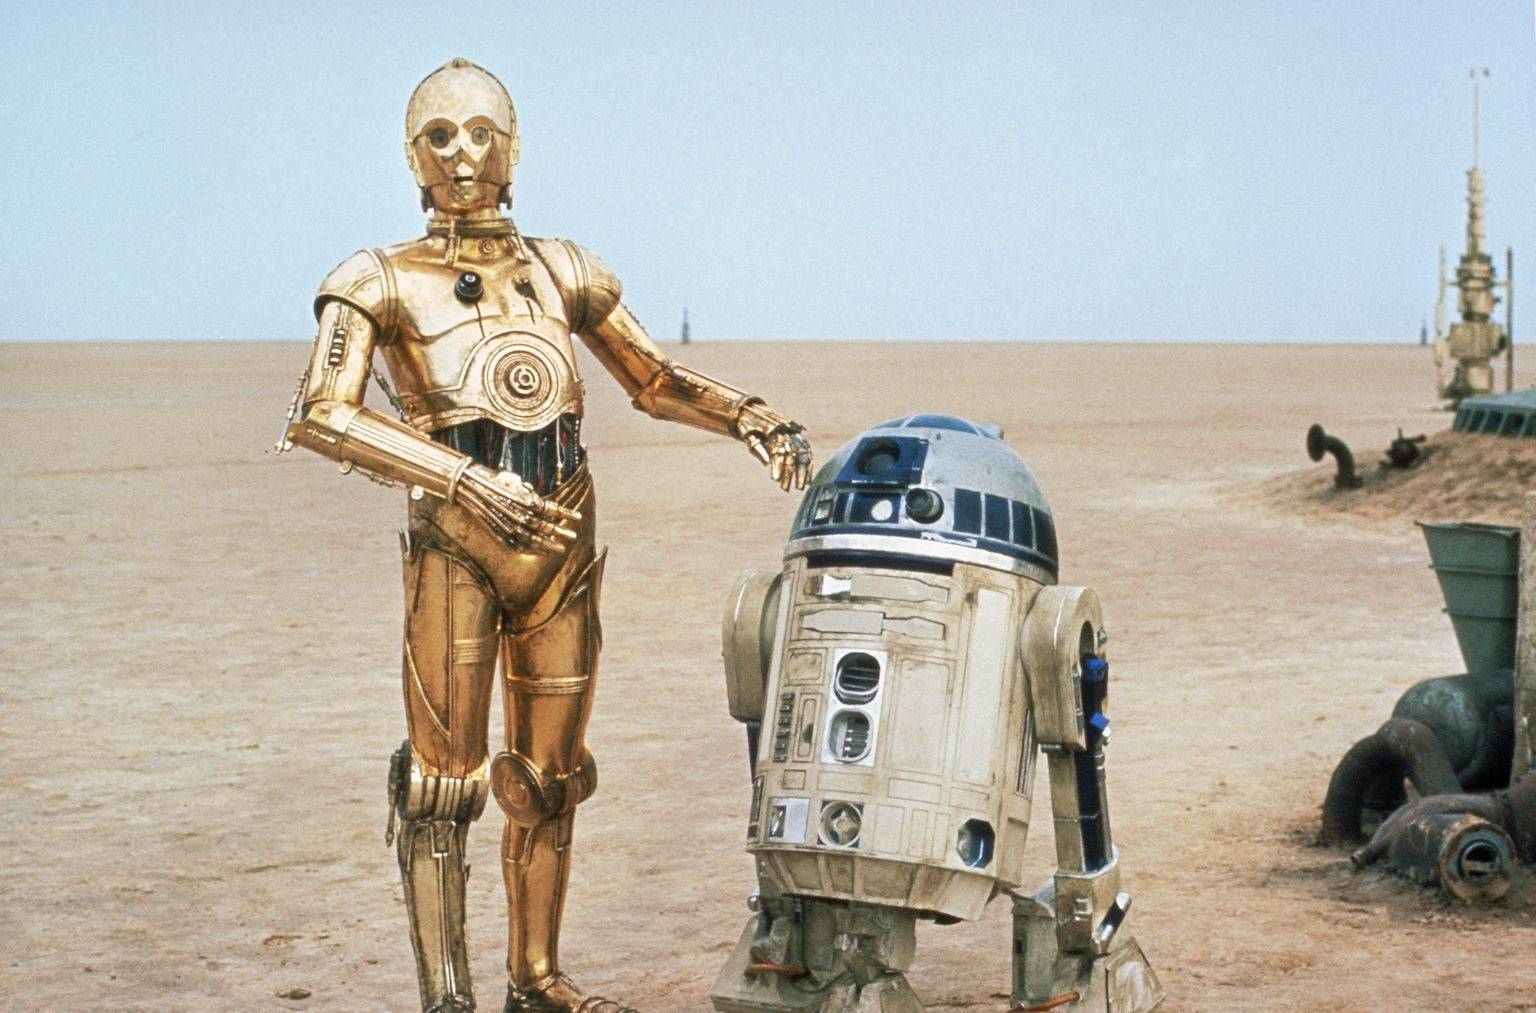
\includegraphics[height=4.5cm]{r2d2.jpg}}
    \hfil
    \subfloat[][Wall-E being curious about a Rubik's cube]{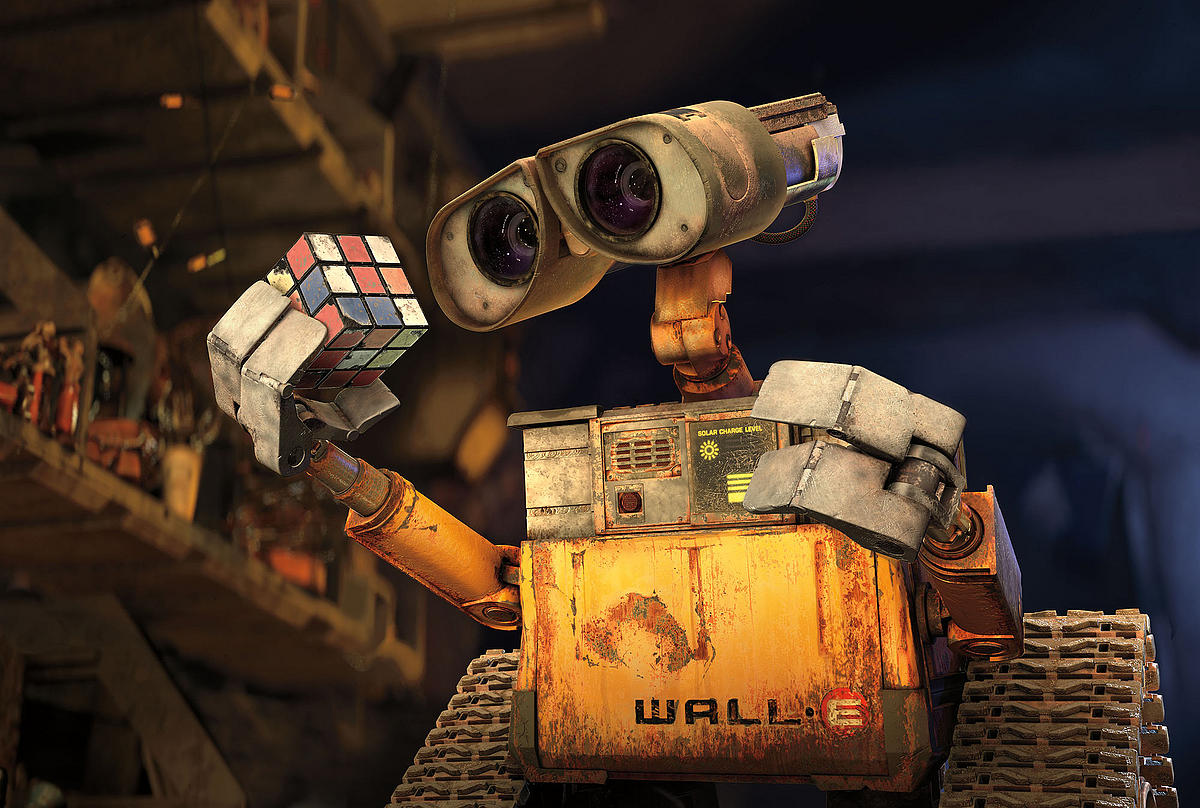
\includegraphics[height=4.5cm]{Wall-E.jpg}}
    \caption{}
    \label{fig:robot_emotion_cinema}
\end{figure}


\section{Motivation } % (fold)
\label{sec:motivation}

Poppy is fully hackable, artists could be interested by the exploration freedom they have such as changing the morphology or the design of the robot, adding new features or sensors, changing its behaviour and so on. Also, Poppy is designed to be experimental-proof (see section REF), it is quite robust and easily reparable so it can be used in rather difficult conditions.

As we discussed previously, the artist community is a rich source of inspiration and can provide new perspectives to scientific and technological questions. The work of artist is complementary to the one of scientific. In the open source robotic community we are trying to set up, this complementarity is a great opportunity that we want to enforce by making the robot accessible for non-robotic-expert users.

While it is a real desire to make Poppy accessible and useful for the Art community, we needed to get experience of such uses in an actual artistic project to evaluate how relevant Poppy is for artists and what artists can bring into the Poppy project development.


\section{The \emph{Êtres et numérique} project} % (fold)

The first artistic project in which Poppy is involved is entitled "Êtres et Numérique". This contemporary art project focuses on the way to represent and interact with the movement digitally. It is led by the artists\footnote{Comacina Capsule Creative, \url{http://www.comacina.org/}} Amandine Braconnier (mixed media artist) and Marie-Aline Villard (dancer-researcher), and supervised by Thomas Desmaison (Point barre\footnote{\url{http://www.pointbarre.biz/}}) from the Fabrik Pola\footnote{\url{http://www.pola.fr/}}.

\begin{figure}[t]
    \begin{center}
        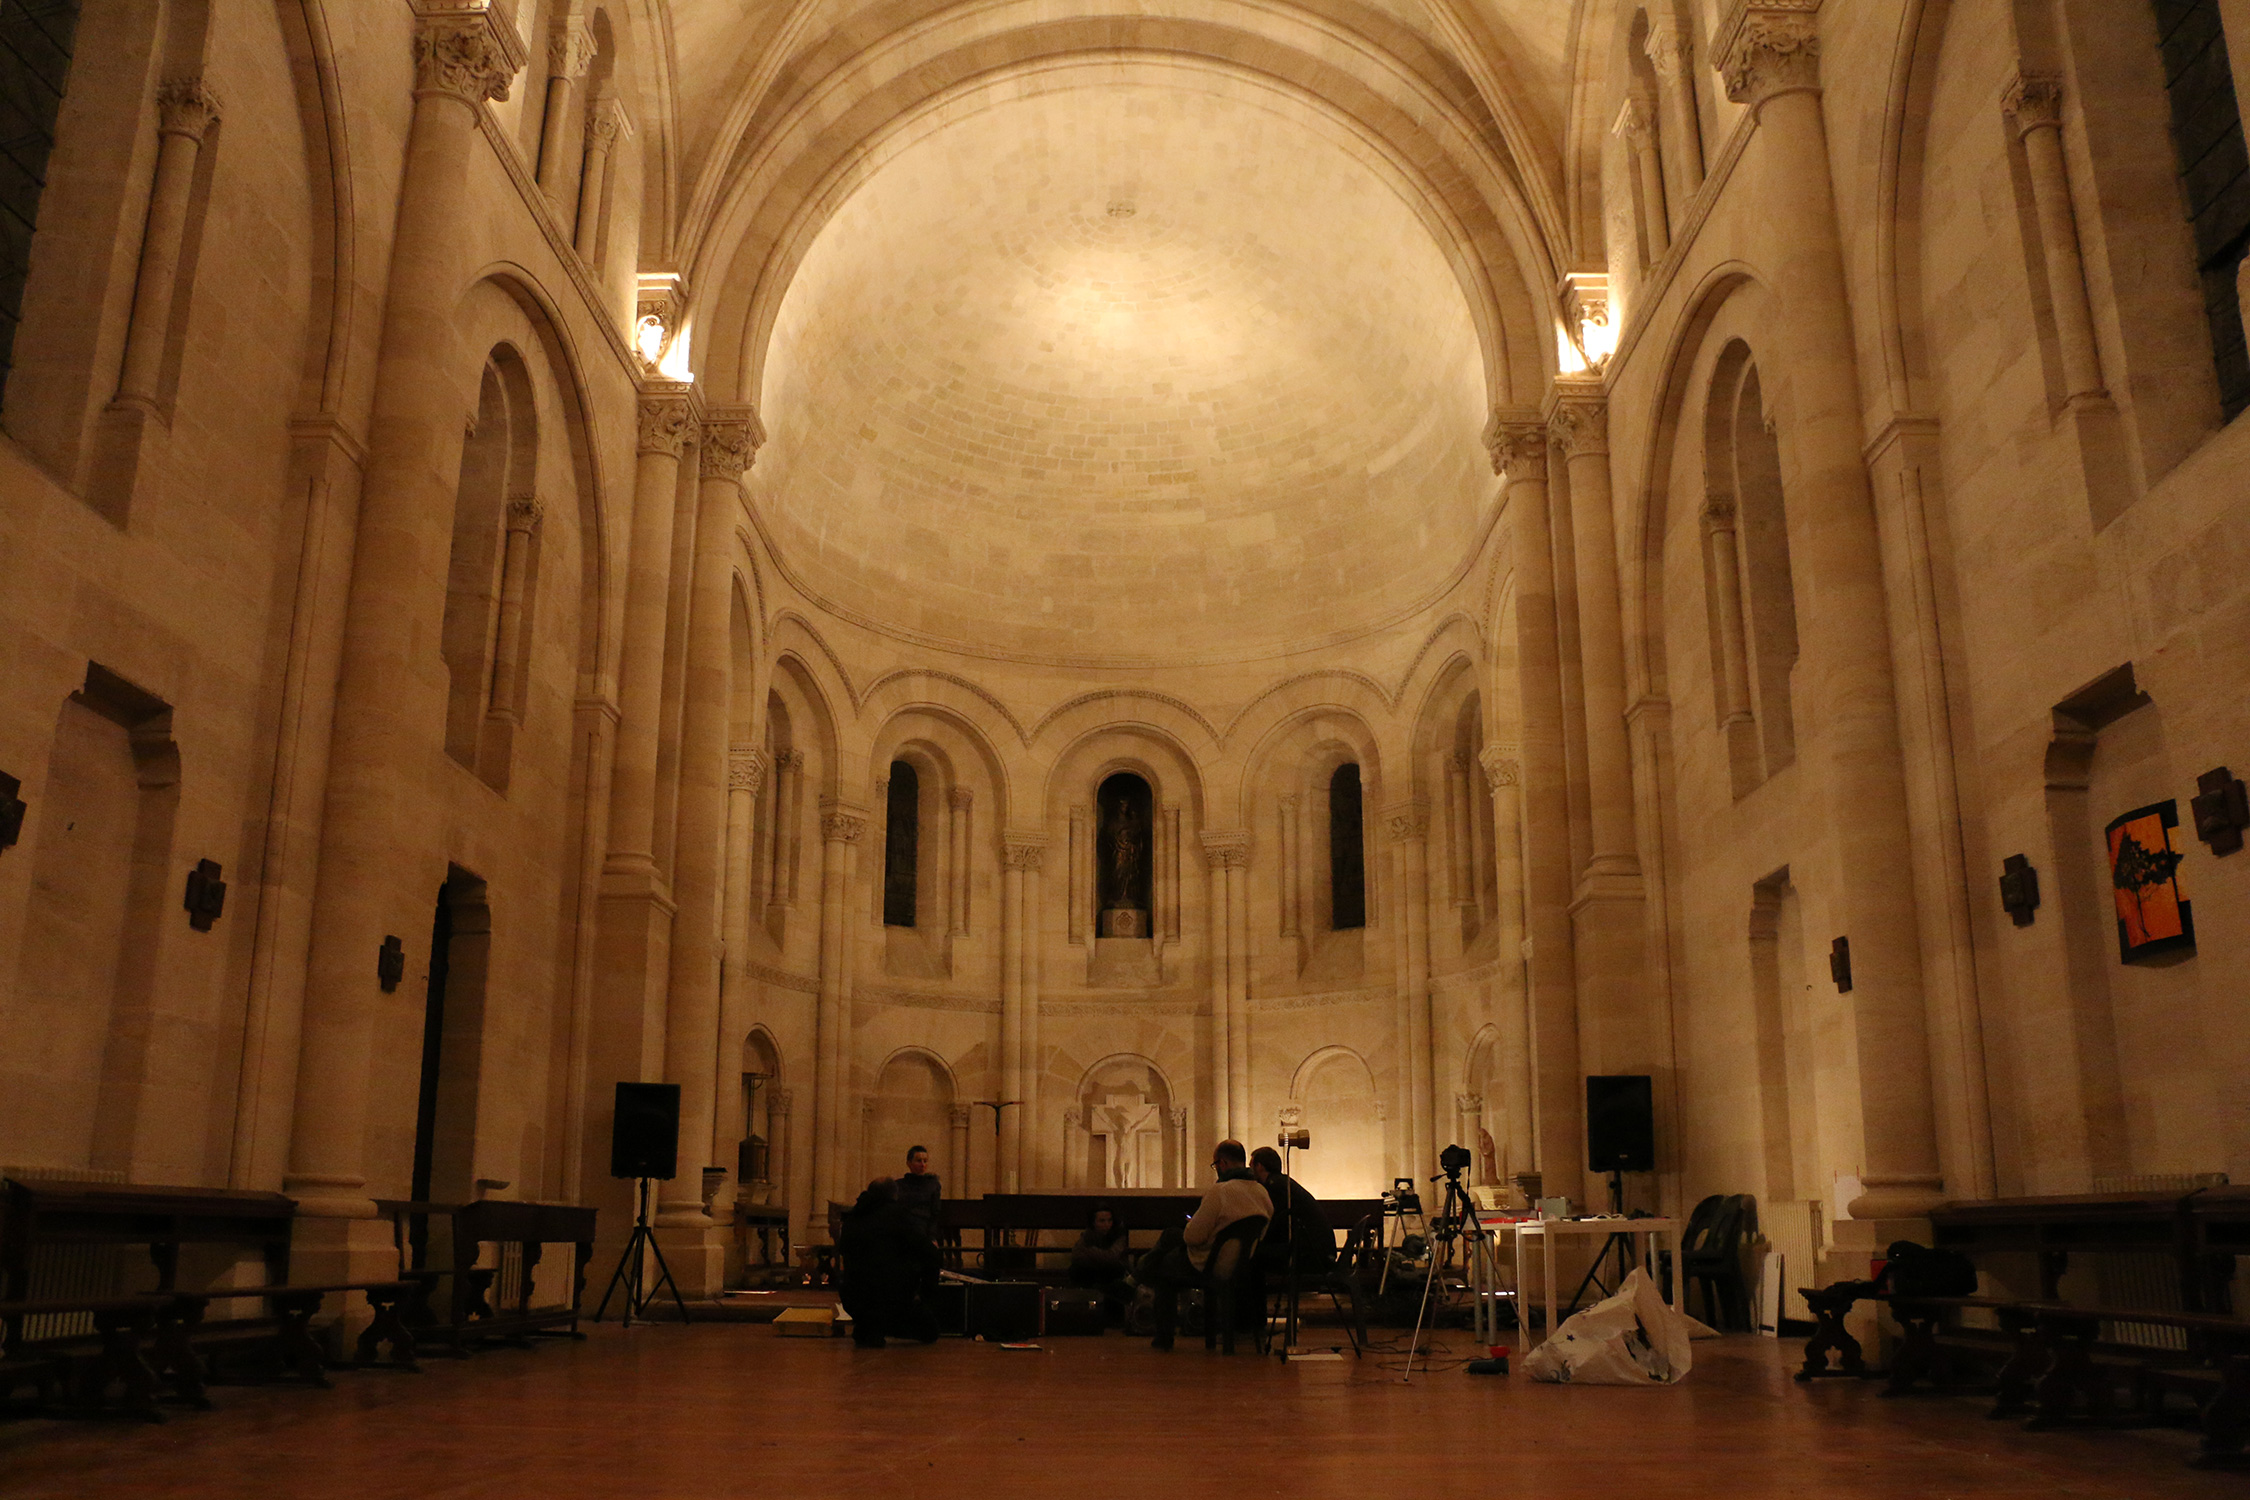
\includegraphics[width=0.8\linewidth]{saintonge_chapel.jpg}
    \end{center}
    \caption{The "Êtres et numérique" residency and performances took place in the gorgeous chapel of the \emph{lycée des metiers Sainte Famille Saintonge}}
    \label{fig:saintonge_chapel}
\end{figure}

\textbf{A video trailer is available here: \url{https://vimeo.com/92281019}.}

For these artists, the use of an hackable humanoid robot is a whole expressive tool opening new horizons. Indeed, a robot permits to dissect and analyse movements. It permits to play with its body and model motions as one could sculpt shape in clay. Also, the use of non-rigid actuation allows the emergence of unpredictable and unexpected movement while the fact Poppy is under-actuated ensures safe physical interaction.


The first "Êtres et Numérique" work took the form of a ten days art-science-mediation residency involving members of the Poppy project, the artists with the participation of Jean Marc Weber (music composer) and was supported by the Aquitaine Région. It took place in a Bordeaux(Fr) high school (Lycée Saintonge Sainte Famille\footnote{\url{http://www.lyceesaintefamille.com/}}), which offers its gorgeous chapel (see \figurename~\ref{fig:saintonge_chapel}) for art performances.


This residency was really important for the poppy project: it was the first trial of a real artistic application with Poppy raising new potential applications and bugs.

The main objective of this first residency was the preparation of a dance performance using passive properties of Poppy and physical human-robot interaction with the dancer, but several experiments has been conducted aside this common thread.


\subsection{Artistic exploration} % (fold)

The residency week was an exploring playground for Poppy and us. Artists were especially interested by the way to represent the movement and the interaction between human and robot.

A first experiment consisted in visually tracing over a canvas the movement combined of the dancer and the robot (see \figurename~\ref{fig:residency_canvas}). To do so, we dressed Poppy to protect it against dirt (see \figurename~\ref{fig:poppy_dressed}). Then M.A Villard danced with Poppy on canvas covered with pigments (see \figurename~\ref{fig:poppy_playing_with_pigment}). These dancing movements have been captured by pigment traces and have created kind of paintings (see \figurename~\ref{fig:pigment_traces}). The whole collection as been exposed in the chapel (see \figurename~\ref{fig:whole_canvas_collection}.

\begin{figure}[tb]
\centering
    \subfloat[][Poppy dressed to protect it against dirt]{\label{fig:poppy_dressed}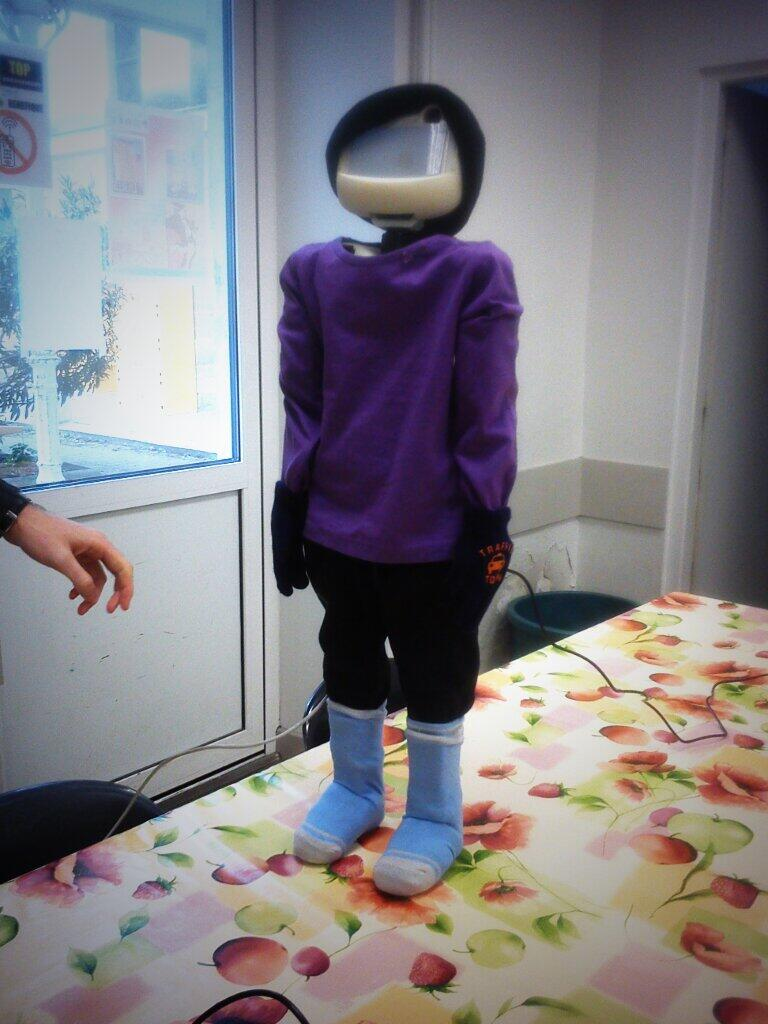
\includegraphics[height=6cm]{poppy_4ans.jpg}}
    \hfil
    \subfloat[][Poppy and the dancer playing on canvas covered with pigments]{\label{fig:poppy_playing_with_pigment}\includegraphics[height=6cm]{IMG_0191.jpg}}\\
    \subfloat[][Result of this human-robot interaction]{\label{fig:pigment_traces}\includegraphics[height=6cm]{_MG_7996.jpg}}
    \hfil
    \subfloat[][The whole canvas collection has been exposed in the chapel]{\label{fig:whole_canvas_collection}\includegraphics[height=6cm]{IMG_0518.jpg}}
    \caption{Movement }
    \label{fig:residency_canvas}
\end{figure}

An alternative way to represent movement can be by transforming motion into sounds. This is the playground of Jean Marc Weber, an electro-acoustician and music-composer, creating music using the interaction between probabilistic composer and body space motions. To do so, he created plugins allowing the use of webcam, Kinect or Leap motion with the music-software Usine\footnote{usine TODO}. For this purpose we explored both the use of Kinect and Leap motion with Poppy.

When Poppy is dressed it can be tracked by Kinect sensor\footnote{A video was taken during tests and is accessible here: \url{https://www.youtube.com/watch?v=VVjBVTtPkFE}}, also thanks to its hands using human shape, it can also play with the Leap motion (see \figurename~\ref{fig:poppy_playing_leap}).

\begin{figure}[tb]
\centering
    \subfloat[][Poppy playing music with Leap motion device]{\label{fig:poppy_playing_leap}\includegraphics[height=6cm]{IMG_0049.jpg}}
    \hfil
    \subfloat[][Poppy playing music with Kinect]{\label{fig:poppy_playing_kinect}\includegraphics[height=6cm]{IMG_0258.jpg}}
    \caption{}
    \label{fig:}
\end{figure}

Finally, Amandine Braconier (Plastic artist) wanted to make an experiment with a little child (3 years). In this experiment, the child can modify the robot appearance by adding clay on it (see \figurename~\ref{fig:clay_on_poppy}). To protect Poppy, we wrapped it with cellophane.

\begin{figure}[tb]
\centering
    \subfloat[][Poppy covered with cellophane ready to be modify using clay]{\includegraphics[width=0.49\linewidth]{IMG_0381.jpg}}
    \hfil
    \subfloat[][Little boy playing while Poppy is silently suffering from all the extra weight put on it.]{\includegraphics[width=0.49\linewidth]{_MG_8034.jpg}}
    \caption{}
    \label{fig:clay_on_poppy}
\end{figure}

This experiment last about 2h and the clay is really heavy. It turns out to be playful for the little boy to put as much clay as possible. Eventually he managed to put almost 10kg on the poor Poppy\dots

On this point, Amandine Braconier says:
\begin{quotation}
    How to use Poppy? The robot is put to the test. I do not know in advance what will happen. Each experiment is photographed and filmed. Some sequences are mounted. I try to emerge from other movements that have not been calculated by the researchers. For example, I suggested an interaction with the robot: a child, through the game, evolves with Poppy. It is in a back and forth continuously between the two actions that the child and the robot meet, separate and detached. In the exchange that occurs remains a singularity and shows a confusion. On the video, we see the child cover the with clay the robot. It transforms it. It gives it a monstrous appearance. Also, the action of the child on the robot causes his downfall. The robot is as if exhausted. We do not know which of the two is the monster. The effect goes far beyond the game. The aim here is to choose what we will do with Poppy and how we will show it.
    \signed{Amandine Braconier (06/18/2014)}
\end{quotation}


\subsection{The dance performance} % (fold)

The common thread of this residency was the work on a contemporary art dance performance involving poetic choreography, alternating phases of autonomous robot movements and passive robot movements provoked by the dancer. Marie Aline Villard describes her work as:

\begin{quotation}
    As a dancer, shared this experience with Poppy movement was very interesting on both the artistic and functional/mechanical aspects. On one hand, I liked working on the line between that animates who, trying to give the illusion of a duet. But on the other hand, I am also amused to show that Poppy was still an object by playing on active/passive and by manipulating genuinely. This edge is a great discovery and artistic research should continue in this direction.
    Also sharing the movement with robotic object remains fascinating, since we project our own movement patterns. I could check during a workshop, at which point we were planning our own move on the structure of the robot. By asking students to make movement between a posture A and a posture B, in spite of themselves they began moving, dancing, just to record a movement for the robot, which leads me to say that Poppy has dis-inhibiting properties, to exploit in the interaction and that dance can greatly contribute.

    \signed{Mari-Aline Villard (Dancer) on the use of Poppy for artistic project}
\end{quotation}

The choreography has been "sculpted" by Marie Aline Villard using the pypot feature to record motion trajectory directly by physical demonstration. Rather than coding, this "direct programming" feature allowed the dancer to express her idea with her language i.e. the movement. Thus she managed to create a whole floor choreography where Poppy slowly moves with elegance and sensibility.
Other scenes were improvised dance with physical interaction and guidance where Poppy was alternatively active or passive.

The whole performance with the several scenes (see \figurename~\ref{fig:poppy_dance_performance}) last about 20 min and has been showed in front of a public audience for the last day of the residency (with about a hundred people). Despite the problems we have had during the residency, Poppy acted really great and no technical problems occurred during the whole performance (repeated 4 times in a row without any interruption)

\textbf{A complete performance set can be seen here: \url{http://youtu.be/zp-vsVQcAvs}.}

\begin{figure}[p]
\centering
    \subfloat[][]{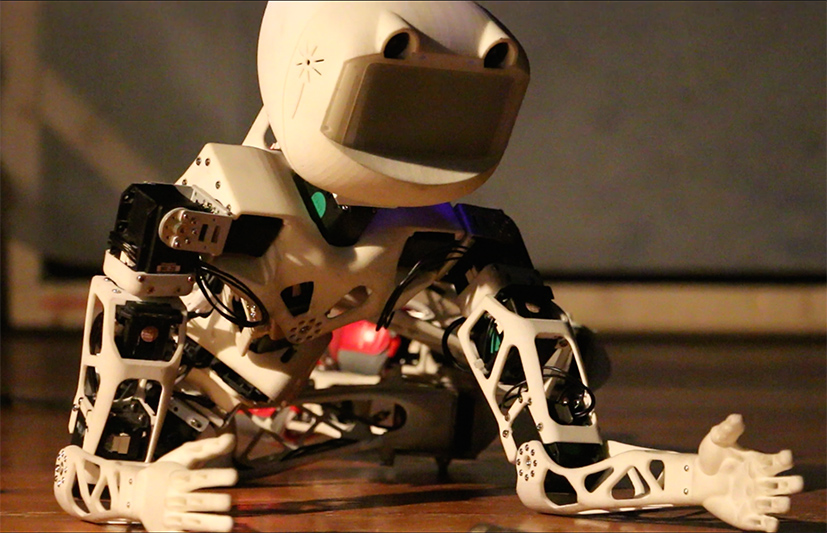
\includegraphics[width=0.46\linewidth]{ENP_img2.png}}
    \hfil
    \subfloat[][]{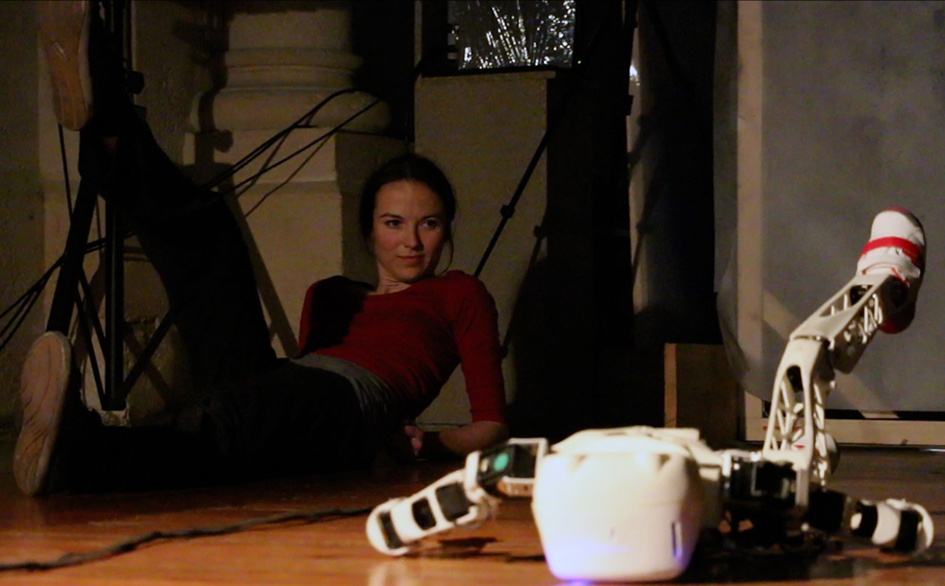
\includegraphics[width=0.46\linewidth]{art_floor.jpg}}\\
    \subfloat[][]{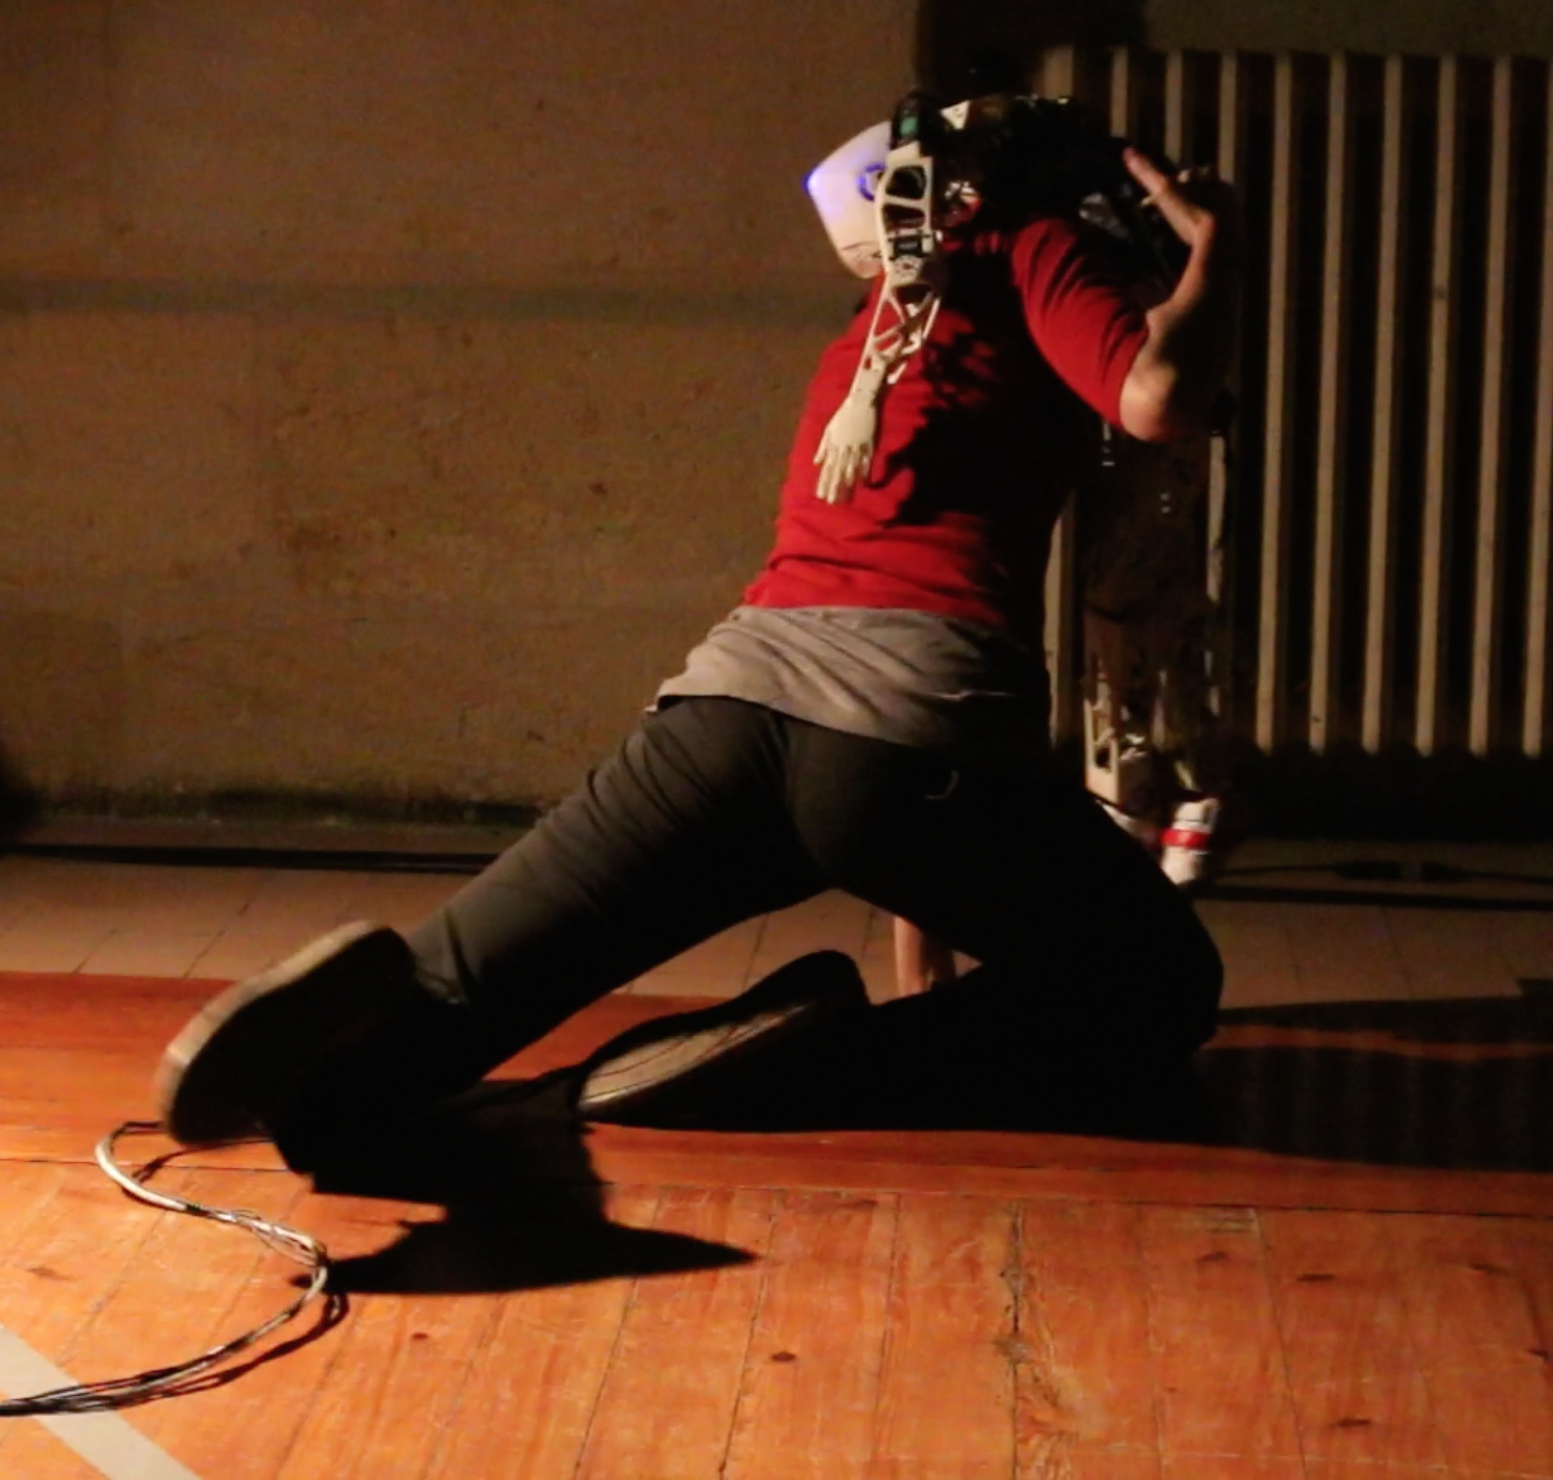
\includegraphics[height=5.3cm]{img6.png}}
    \hfil
    \subfloat[][]{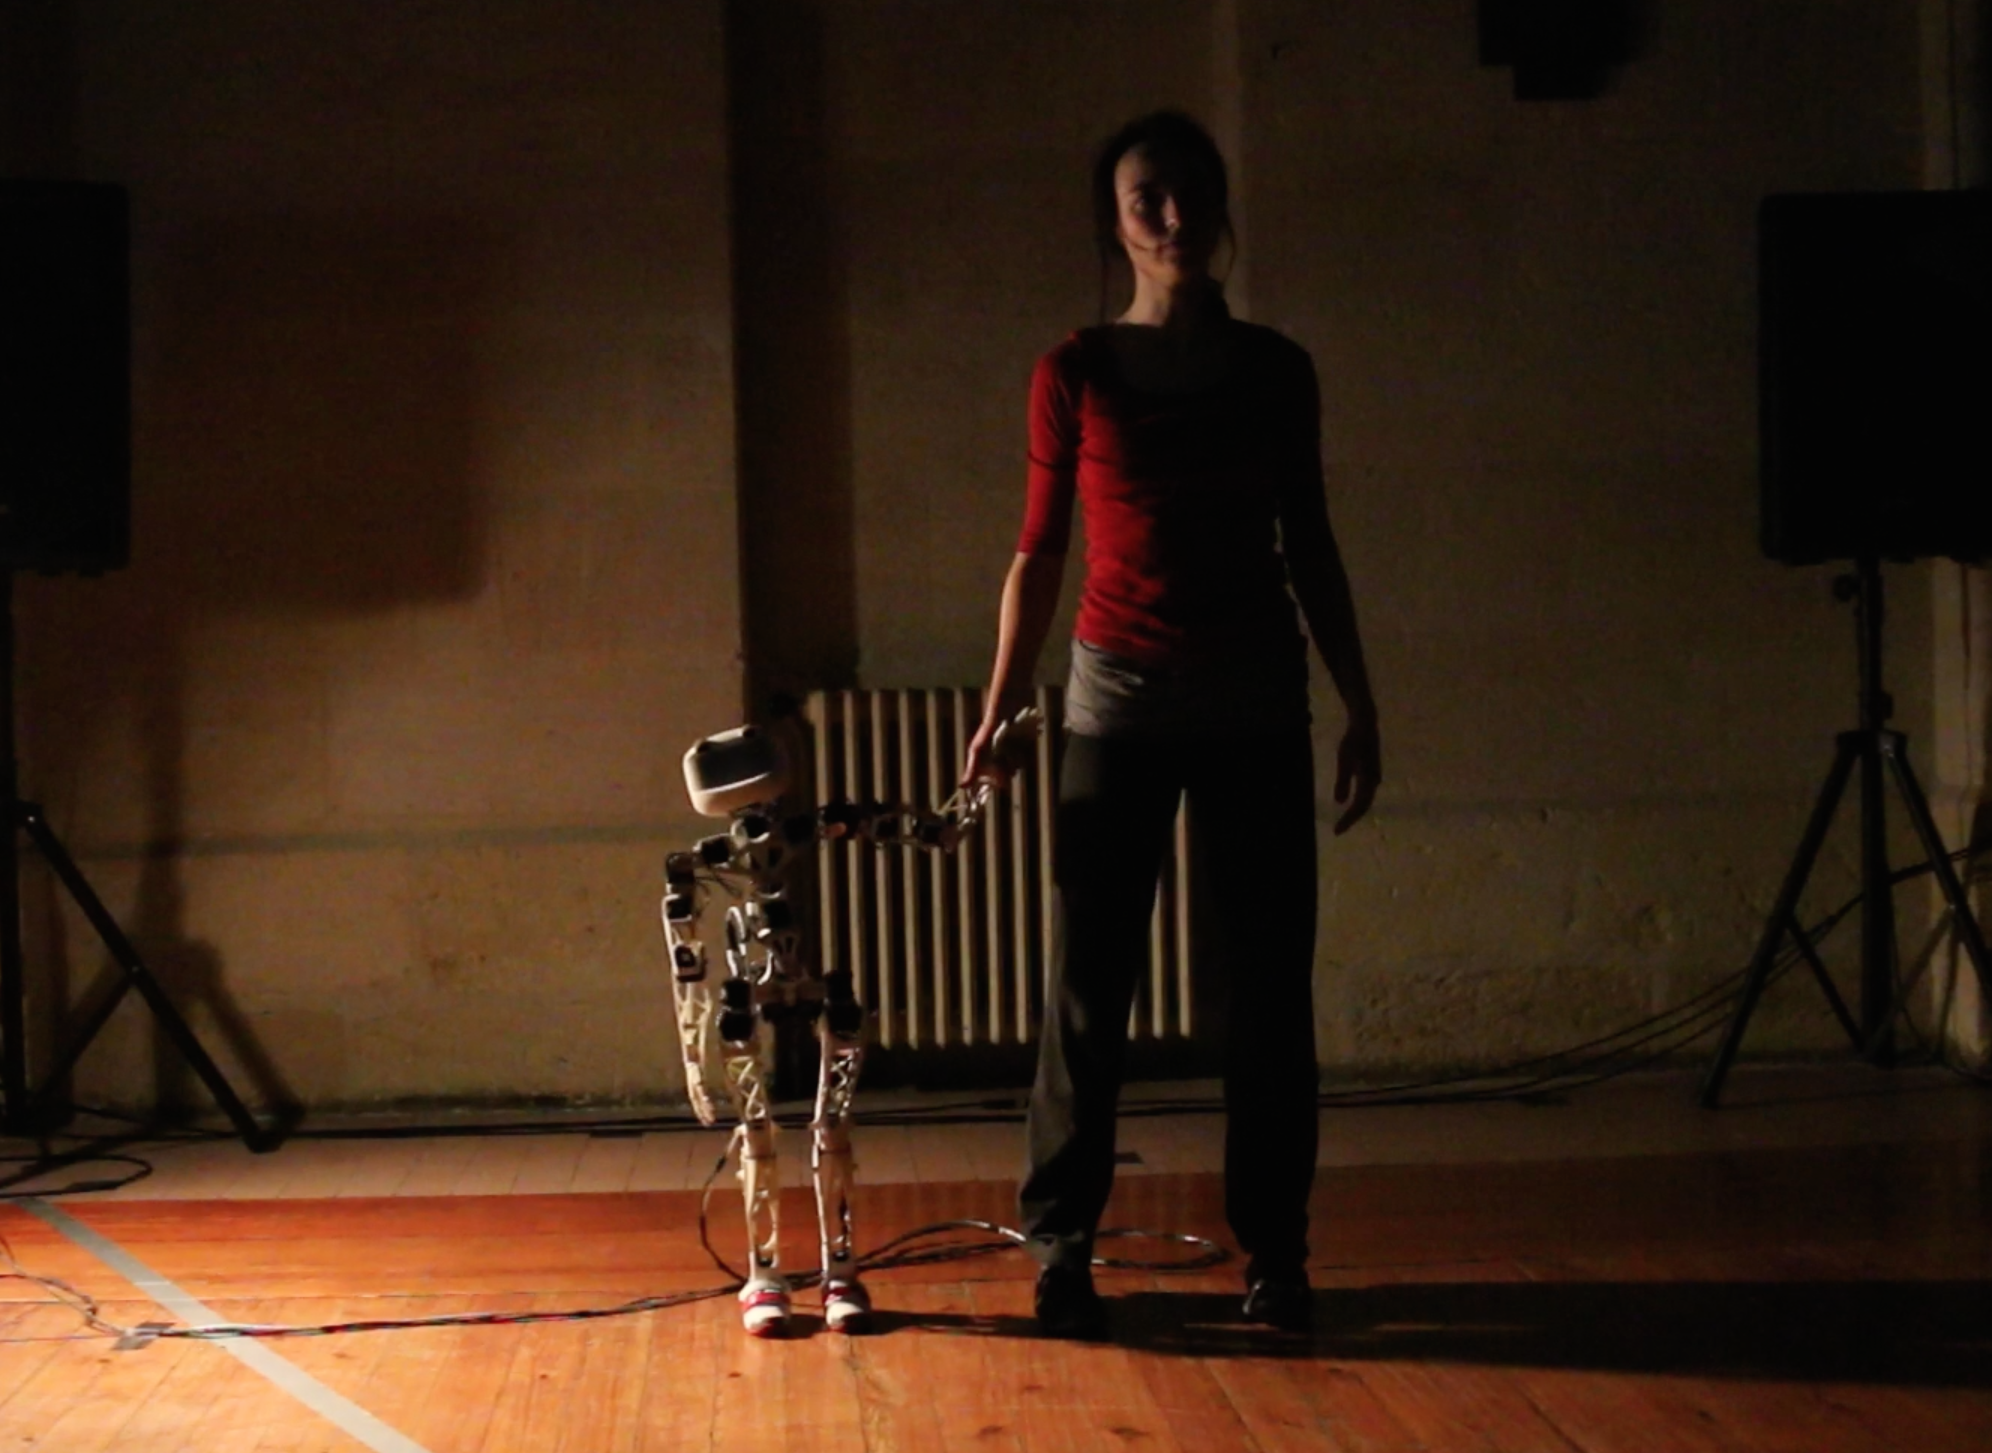
\includegraphics[height=5.3cm]{poppy_dancer_stand_up.png}}\\
    \subfloat[][]{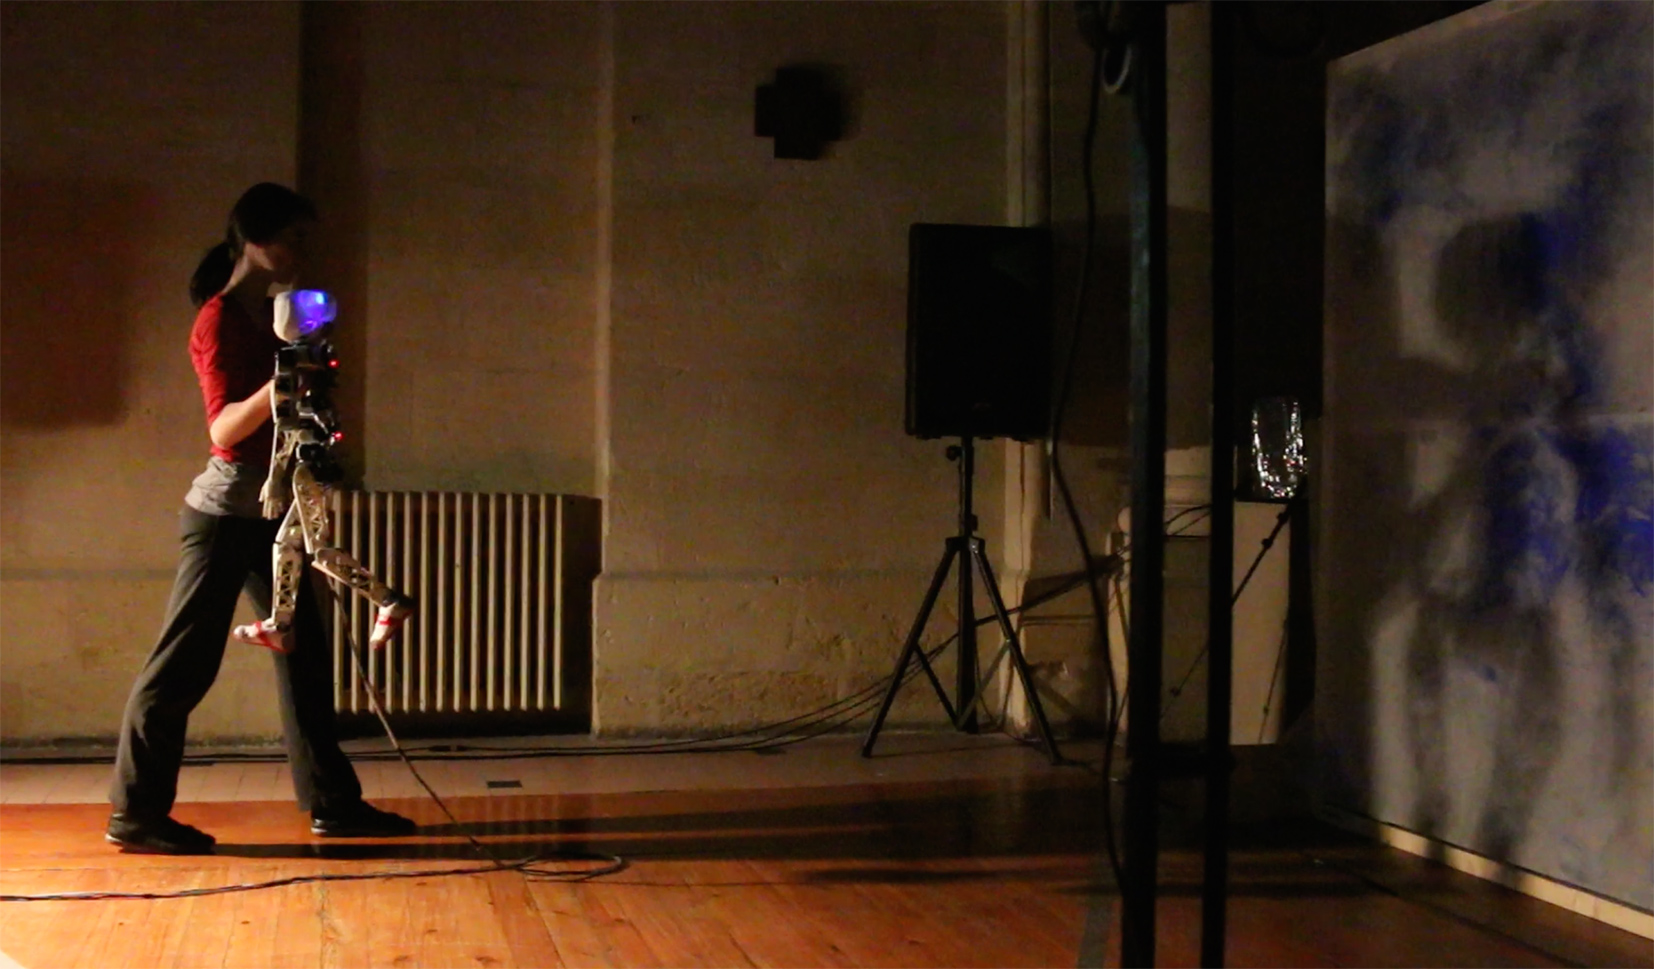
\includegraphics[width=0.95\linewidth]{img3.png}}
    \caption{}
    \label{fig:poppy_dance_performance}
\end{figure}


\subsection{Feedback} % (fold)

Unfortunately or fortunately, all these workshops did not occurred without problems with the use of Poppy by artists (\figurename~\ref{fig:broken_poppy_residency}).

First, it appears it is difficult for non-expert user to evaluate the actual resistance of Poppy. After some times acting really preciously with it, they get confident about its robustness and do not pay attention no more to signs indicating the robot is going to be broken. The experience with the little boy putting clay has been quite destructive. Poppy spent almost 2 hours in cellophane supporting kilos of clay, eventually it overheated and two motors in the hip and abs have melted.
Thus it appears really needed to add security system raising alerts when the robot is in a dangerous state.  Otherwise non-expert people will break regularly motors without understanding why.

\begin{figure}[]
\centering
    \subfloat[][]{\includegraphics[height=4.5cm]{IMG_0019.jpg}}
    \hfil
    \subfloat[][]{\includegraphics[height=4.5cm]{IMG_0046.jpg}}
    \caption{}
    \label{fig:broken_poppy_residency}
\end{figure}

Second, the strong interaction between Poppy and the dancer showed it was really complicated, when the robot is compliant, to avoid motors to go on their dead-band. In addition, wires tend to tangling around motors, which eventually unplug some of them. To avoid this recurrent problem, we built a pypot primitive checking the state of each motor and stopping it when it reach a given amplitude. Also, we are working on mechanical way to avoid full-rotation of certain Poppy links.

Third, the wire are really problematic, they caused a lot of problem along the residency. In this context of intensive use of the robot doing large amplitude motion, wires have been solicited and eventually some of them began to be damaged which provoked short-circuit and so destroyed some motors and micro-controller.

During the residency, the ease of programming through the Pypot library permitted to design a simple interface allowing the dancer to physically sculpt novel movements, which softness could be dynamically controlled.

The pypot programing by demonstration is really basic, position are recorded at 50hz and played. It is not at all optimized and yet a bit annoying to use because you cannot edit your moves. But this way to "program" the robot has also a great advantage. The artist really appreciate to sculpt motion like this rather than editing curve on a nice interface because she can really feel the weight of the robot and work on the way to move its mass from one support to another. Finally, because Poppy is not over-actuated, it constrains motion to whom requiring the less power actuation and therefore leads to the creation of more natural motion.


\section{Discussion} % (fold)

The work the artists did, was really amazing and they find unexpected potential in Poppy. Among them, the choreography Marie Aline Villard did, was very elegant and sensible. These movements put Poppy in a sensible domain rarely saw in humanoid robotics. This choreography is now often used for demonstration of the Poppy platform and closes the communication video showing Poppy being assembled in time-lapse \url{https://vimeo.com/96262428}.
Also, from a community impact point of view, the topic\footnote{\url{https://forum.poppy-project.org/t/artist-residency-etres-et-numerique/}} related the experience is by far the most followed subject of our forum.

But this work showed also the limit of Poppy. As the Ergo-robots experience\footnote{Ergo-robots had to be functional for 5 months 8h/day. Our technologies have been really confronted for long-term experiences in the real world. In particular, the feedback we get from this experience greatly contribute in the methodology we have built for the design of Poppy.}, the artist residency around Poppy we had has been really instructive. First, Poppy has been used in totally unknown and unexpected/able situations, playing in pigments, dancing 2h long and so on were not on the development to-do list.
It was a real crash test for a novel experimental platform. Again, like in the ergo-robot experience, we learn the hard way how problematic are the wires. Most of the problem we had was due to damaged wires, which provoked short-circuit and eventually destroyed some motor and micro-controller. It is a real problem in robotic right now, and it is really complicated to find a way to avoid it while keeping a modular et highly hackable robot.

We took note of each hardware problem to be solved for the release of the 1.0 version of Poppy and they are in progress. Yet it will maybe not enough (at the beginning) because it appears we need to add also specific software to monitor and protect the robot motors against overheating and overload. These protections are often task-dependent and the way we should handle it remains unclear. Therefore the development will be done with the community in an iterative way until finding an efficient and robust solution.

Another problem for the diffusion in the Art community is the cost of the robot. Obtaining the 7000-8000\texteuro required to build a Poppy is really difficult and Artists already having difficulty being paid so they have few founding for material.

An alternative could be to rely on the growing Fablab community~\cite{anderson}. The collaboration between an artist and a Fablabs could permit at the same time to ensure a technical support and assistance for using Poppy, avoid the funding problem by using Fablab's Poppy and promote local collaboration between complementary actors.

The interaction with Fablab is a very important point for the Poppy project, we will discuss it in the next chapter.

